\section{U005 Tail axis reductions and the placement of partial state}
\label{sec:u005}

\subsection{The logical axis does not determine the physical reduction}

For a logical array $X\in\mathbb{R}^{G\times K}$, a row sum produces $G$ outputs,
\begin{equation}
 y_g=\sum_{j=0}^{K-1}X_{g,j},\qquad 0\leq g<G.
 \label{eq:u005-logical}
\end{equation}
This notation omits the order and precision of additions. It also says nothing about whether a row belongs to one thread, several SIMD lanes, a vector register, multiple tiles, or several cores. Those ownership choices determine the exchanges and partial storage needed to form $y_g$. The tail axis is often physically contiguous, which can simplify reading values, but contiguity does not imply that all of them reach one accumulator without communication.

There are two distinct sources of parallelism. Different $g$ values are independent unless the surrounding algorithm introduces another dependency. Within one row, reassociation may allow a parallel tree, but only if the numerical contract permits it. A binary tree combining $K$ values has $K-1$ combines and ideal depth $\lceil\log_2K\rceil$. A prescribed fold can have a dependence through every input. Neither count determines cycles: an instruction may process several rows, the hardware may be pipelined, and communication or operand delivery can dominate arithmetic. Consequently, many short rows and a few very long rows are different architectural cases even when $GK$ is the same.

For a higher-rank array such as $X[B,H,Q,K]$, reducing the last axis leaves independent output coordinates $(b,h,q)$. If their layout permits, they can be mapped to one group index $g$. Rank four does not itself require four reduction levels. Reducing a middle axis is different because the retained and reduced coordinates can be interleaved. Stride-aware iteration, a transpose, or staged accumulation are alternatives; the correct choice depends on traffic, retained state, and available output-level parallelism. A row-major column reduction may simply vectorize across output columns while iterating over rows, so a transpose is not inherently required.

\subsection{A four element group example}

Consider 32 contiguous FP32 input elements partitioned into eight groups of four. The logical operation is
\begin{equation}
 X[8,4]\longrightarrow y[8,1],\qquad
 y_g=\operatorname{reduce}(X_{g,0},X_{g,1},X_{g,2},X_{g,3}).
 \label{eq:u005-four}
\end{equation}
The input contains 128 logical bytes and the output contains 32 logical bytes. These are element counts, not a claim about how many physical allocation bytes either side consumes. In a contiguous RowMajor representation, a 128-byte payload can hold all eight input groups. A blocked matrix layout has a different physical envelope, even when its valid region has the same 32 elements.

The pinned PTO CUBE contract defines each CELL as 128 bytes. For 32-bit elements, a \texttt{CUBE\_M16} CELL has shape $16\times2$, whereas a \texttt{CUBE\_M32} CELL has shape $32\times1$. Thus the four columns of one logical group span two column CELLs in M16 and four in M32. Eight valid rows require the physical envelopes
\begin{align}
 S_{\rm M16}&=16\cdot4\cdot4=256\text{ bytes},\\
 S_{\rm M32}&=32\cdot4\cdot4=512\text{ bytes}.
 \label{eq:u005-envelope}
\end{align}
The extra rows are part of the layout envelope; they are not extra logical groups. It is incorrect to identify every 128-byte CELL with one four-element group or to infer the number of groups executed per cycle from the number that fit in storage. For 16-bit elements the CELL geometries become $16\times4$ and $32\times2$; for 8-bit elements they become $16\times8$ and $32\times4$. These are descriptor and storage facts, not arithmetic-width or service-rate guarantees.~\citep{u005-pto-cell}

\begin{figure}[tb]
\centering
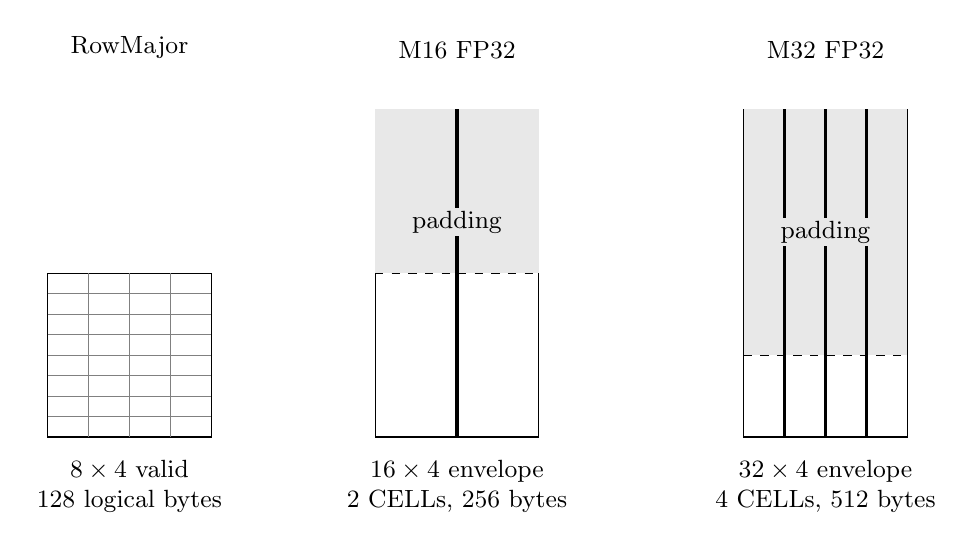
\begin{tikzpicture}[x=0.52cm,y=0.26cm,font=\small]
 \foreach \x/\lab in {0/{RowMajor},8/{M16 FP32},17/{M32 FP32}} {
  \node[anchor=south] at (\x+2,18) {\lab};
 }
 \draw (0,0) rectangle (4,8);
 \foreach \y in {1,...,7}{\draw[gray] (0,\y)--(4,\y);}
 \foreach \x in {1,2,3}{\draw[gray] (\x,0)--(\x,8);}
 \node[align=center] at (2,-2.4) {$8\times4$ valid\\128 logical bytes};
 \draw (8,0) rectangle (12,16);
 \fill[gray!18] (8,8) rectangle (12,16);
 \draw[very thick] (10,0)--(10,16);
 \draw[dashed] (8,8)--(12,8);
 \node[align=center] at (10,-2.4) {$16\times4$ envelope\\2 CELLs, 256 bytes};
 \draw (17,0) rectangle (21,16);
 \fill[gray!18] (17,4) rectangle (21,16);
 \foreach \x in {18,19,20}{\draw[very thick] (\x,0)--(\x,16);}
 \draw[dashed] (17,4)--(21,4);
 \node[align=center] at (19,-2.4) {$32\times4$ envelope\\4 CELLs, 512 bytes};
 \node[align=center,fill=gray!18,inner sep=1pt] at (10,10.5) {padding};
 \node[align=center,fill=gray!18,inner sep=1pt] at (19,10) {padding};
\end{tikzpicture}

\caption{The same eight groups of four FP32 values in three representations. Each diagram has four logical columns; M32 rows are drawn at half the vertical scale. Shading denotes physical rows outside the valid region. CELL divisions describe storage, not execution cycles.}
\label{fig:u005-cells}
\end{figure}

The result also needs an allocation contract. The pinned row-reduction specification creates a new Local destination and preserves its source. The destination has one \emph{valid} column. For CUBE M16/M32 it retains the source's physical column envelope and uses the minimum legal physical row envelope covering the valid rows. In this example, the logical result therefore remains eight FP32 values, but a CUBE destination with four physical columns still carries the 256- or 512-byte envelope above. RowMajor derives its physical rows from the selected destination capacity and one column; its allocation is also not proved to be 32 bytes merely by counting results. A later compaction or layout conversion may reduce storage if the ISA and allocator support it, but that operation and its lifetime must be accounted for. A prefix view alone does not establish that the unused part of an allocation has been returned to the allocator.~\citep{u005-pto-trowsum,u005-pto-reduction-legality}

\subsection{The ordered fold is an architectural constraint}

At PTO revision \texttt{e182c9b}, \texttt{TROWSUM} is selected through the \texttt{TEPL} encoding carrier and dispatched as an SFU block operation. It is not a separate standalone opcode. Its semantic contract is a typed left fold beginning with typed zero, in increasing column order:
\begin{equation}
 a_{g,0}=0_{\tau},\qquad
 a_{g,j+1}=\operatorname{TADD}_{\tau}(a_{g,j},X_{g,j}),\qquad
 y_g=a_{g,K}.
 \label{eq:u005-fold}
\end{equation}
Here $\tau$ is the operation type, including its rounding and status behavior. The contract does not authorize replacing this recurrence by a balanced floating-point tree. Independent groups may run in parallel while each group's observable result and numeric status follow the recurrence. Even then, the actual number of groups processed simultaneously depends on datapaths, ports, issue capacity, and implementation scheduling; it is not given by the semantic definition.~\citep{u005-pto-trowsum}

A concrete FP32 round-to-nearest illustration explains why the distinction matters. For the four inputs
\begin{equation}
 [2^{25},\ 1,\ -2^{25},\ 1],
\end{equation}
the prescribed fold loses the first added $1$ at the large magnitude, cancels the large values, and ends at $1$. A pairing that first forms $(2^{25}+1)$ and $(-2^{25}+1)$ rounds both pairs to the large signed powers of two and then obtains $0$. The real-arithmetic sum is $2$. This example is a derived numerical illustration, not a benchmark or a claim about another architecture's default reduction mapping. It shows that ``four inputs, two tree levels'' is not a legal optimization merely because it looks like the same mathematical sum.

The initial addition from typed zero is also part of the defined operation. An implementation may simplify it only when it preserves the type's full observable semantics, including exceptional inputs and status. Integer addition in the pinned contract retains element-width bits at each step; no separate wider accumulator is implied. The input carrier can be an equal-width non-packed view where the contract permits, but a view is an interpretation, not an arithmetic conversion. An FP32 matrix accumulator elsewhere in the architecture does not grant FP32 accumulation to a typed FP16 reduction.

There is a further implementation boundary. The pinned legality list admits types whose floating fold helper does not yet define an element result: the public reader guidance identifies TF32, HF32, E4M3, and E5M2 as reaching an incomplete \texttt{ScalarFPBinaryProfile} path. The article therefore does not present FP8 sum as an established complete executable capability. A type name in the legal-type list and a complete numeric implementation are separate evidence. Resolving this gap requires a specified arithmetic profile and validation, not merely adding an instruction name to a table.~\citep{u005-pto-trowsum}

\subsection{Masks, padding, and incomplete groups}

The current reduction contract includes every coordinate in the valid source rectangle. It rejects the generic Local CUBE ExecutionMask, including mask state supplied directly to the model. This is different from the shared PE mask: an all-zero PE mask is a strict no-op at a coarser participation boundary. The PE mask cannot be substituted for arbitrary per-element reduction participation. These rules prevent an implementation from silently treating a general element mask as a supported ragged reduction.~\citep{u005-pto-reduction-legality}

For a flat length $N$ grouped by four, let $G=\lfloor N/4\rfloor$ and $r=N\bmod4$. The $G$ complete groups have shape $[G,4]$. If $r\ne0$, the final group requires separately defined handling: a smaller legal shape, a distinct scalar/vector path, or explicitly materialized identity values under a numerical contract that permits them. Padding \emph{outside} a valid rectangle does not make those elements participants in the reduction. Conversely, extending the valid rectangle and filling it with zeros changes which typed operations occur. Such a change must preserve the required rounding, signed-zero, NaN, and status behavior rather than relying only on a real-arithmetic identity.

The same issue appears in masked softmax. An inactive logit is often represented by a suitable negative infinity before the maximum and exponential stages, but the behavior of an all-masked row must still be chosen. A sum's identity, a maximum's identity, and the output policy for an empty normalization are different decisions. The current nonzero-dimension requirement also means an empty Tile cannot be assumed to encode an empty reduction with a convenient default result. Compiler-generated tails have to respect these legality and result rules.

\subsection{Four PE local reductions and a shared Tile Register merge}
\label{sec:u005-four-pe}

Four processing elements (PEs) can cooperate in two fundamentally different ways. First, each PE can own complete, independent reduction groups. For the eight groups of four in Equation~\ref{eq:u005-four}, assign groups $0,1$ to PE~0, groups $2,3$ to PE~1, and so on. Each PE produces two final group results. No cross-PE combine is needed to compute those eight answers, although distributing inputs and handing results to their eventual consumers can still require movement and synchronization. This mapping exposes parallelism \emph{between} groups without changing the prescribed arithmetic \emph{within} a group.

Second, the four PEs can own disjoint subsets of the \emph{same} global group. If one row has $K$ inputs and PE~$p$ owns the subset $I_p$, then a local reduction produces a partial $s_p$. Under a numerical contract permitting this decomposition, the logical construction is
\begin{equation}
 s_p=\operatorname{reduce}_{j\in I_p}(X_j),\qquad
 y=\operatorname{merge}(s_0,s_1,s_2,s_3),
 \quad \biguplus_{p=0}^{3} I_p=\{0,\ldots,K-1\}.
 \label{eq:u005-pe-partials}
\end{equation}
Four local answers are not four final answers to that one global reduction. A consumer needing $y$ must obtain the contribution from every required participant. Different ownership of the same logical axis changes the communication requirement, even when the local reduction instruction is unchanged.

The proposed target architecture makes a shared Tile Register available as a handoff location for PE-produced values. Its intended role here is to let a larger reduction be partitioned across PEs, locally compress each partition, publish those smaller partials, and read them for a final merge. This is a \emph{target-design discussion}; the present source inspection does not demonstrate a particular physical shared-register topology, port count, merge datapath, throughput, or synchronization implementation. ``Shared Tile Register'' names the intended visible handoff resource, not a measured zero-latency or infinitely multiported structure.

\begin{figure}[tb]
\centering
\begin{tikzpicture}[x=1cm,y=0.8cm,font=\small,>=Latex]
 \node[anchor=west,font=\small\bfseries] at (0,5.4) {Independent complete groups};
 \foreach \x/\p/\g in {0/0/{0,1},3.2/1/{2,3},6.4/2/{4,5},9.6/3/{6,7}} {
  \draw[fill=gray!10] (\x,4.2) rectangle (\x+2.7,5);
  \node[align=center] at (\x+1.35,4.6) {PE \p: groups \g};
  \draw[->] (\x+1.35,4.2)--(\x+1.35,3.65);
  \node[align=center] at (\x+1.35,3.35) {two final results\\no reduction merge};
 }
 \node[anchor=west,font=\small\bfseries] at (0,2.35) {One global group split across four PEs};
 \foreach \x/\p in {0/0,3.2/1,6.4/2,9.6/3} {
  \draw[fill=gray!10] (\x,1.2) rectangle (\x+2.7,2);
  \node at (\x+1.35,1.6) {PE \p: partial $s_{\p}$};
  \draw[->] (\x+1.35,1.2)--(\x+1.35,0.65);
 }
 \draw[fill=gray!18] (0,-0.05) rectangle (12.3,0.65);
 \node at (6.15,0.3) {Shared Tile Register: publish partials and establish readiness};
 \draw[->] (6.15,-0.05)--(6.15,-0.65);
 \draw (2.6,-1.4) rectangle (9.7,-0.65);
 \node at (6.15,-1.025) {Read, merge, and distribute if needed};
\end{tikzpicture}

\caption{Two logical ownership choices for four PEs. The upper path assigns complete groups locally. The lower path needs a cross-PE merge and a numerical contract permitting its partial-reduction order. Input/output movement still exists in the upper case. This target-design diagram specifies neither physical topology nor timing.}
\label{fig:u005-pe-ownership}
\end{figure}

For a long row, local compression can substantially reduce the logical data handed to the merge relative to forwarding every input. For example, four partitions of 256 FP32 values contain 4096 input bytes in total; four FP32 partials contain 16 logical bytes. That arithmetic is only a payload comparison. If all four partials are written to shared storage and read once by one merger, the handoff accounts for 16 logical write bytes and 16 logical read bytes, before physical transfer granularity, padding, metadata, contention, result storage, or broadcast. Keeping the merger's own partial local could avoid one of those shared write/read pairs. The actual traffic and allocation follow the supported Tile and register organization. The earlier CUBE-envelope example is a reminder that 16 logical bytes do not establish a 16-byte physical allocation or shared transfer. Conversely, splitting a four-element group across four PEs leaves one value per PE, so there is no local reduction compression before the exchange; distributing whole short groups may be the more useful mapping.

A shared handoff needs an explicit producer--consumer protocol. Each partial requires a unique group and generation identity, storage ownership, and a rule establishing when its payload is visible. The merge must depend on all required partials, or incrementally combine arrivals while still waiting for the last required contribution before publishing the final result. Reusing a partial's slot must wait until every relevant reader is finished. If multiple PEs subsequently normalize their own input partitions, the final sum, maximum, or reciprocal must also be made available to each consumer. A single merger's completion does not by itself broadcast the result or release every participant's state.

Hardware readiness tracking could enforce these dependencies without software executing a full barrier after every local step. Such an implementation still performs synchronization in the architectural sense: it prevents a dependent read from preceding publication and prevents reuse from preceding consumption. A shared register does not remove those causal edges. It moves their enforcement into a particular combination of descriptors, ready bits, dependency joins, arbitration, and possibly software events. The scope and granularity of publication must also be defined; a reader cannot assume that observing one ready CELL makes all other partials ready.

The cost ledger therefore includes shared-register read/write bandwidth, bank and port conflicts, arbitration, temporary partial storage, readiness joins, the merge engine, and result distribution. If $r_p$ is the time at which PE~$p$'s required partial becomes visible, then publication of a final result using every contribution cannot precede $\max_p r_p$. A merge can overlap earlier work and consume partials as they arrive, but it cannot manufacture the missing slow participant's value. Load imbalance, a delayed input, or contention on one PE can therefore dominate the final dependency. If all four PEs need the statistic, broadcast or repeated reads add another resource demand whose cost depends on the actual fabric.

\paragraph{Exact fold versus distributed reassociation.}
Equation~\ref{eq:u005-pe-partials} is not automatically a legal implementation of the current floating-point \texttt{TROWSUM}. The pinned contract in Equation~\ref{eq:u005-fold} begins from zero and visits columns in order. Independently folding each partition from zero and then merging its sum generally changes rounding and status compared with that global recurrence, even if the partitions are contiguous and the final merge visits them in column order. Passing the running accumulator to the next contiguous partition and continuing the ordered additions can preserve the arithmetic recurrence, using a separately supported sequence or implementation mechanism. Current \texttt{TROWSUM} exposes no seed-accumulator operand. Full instruction equivalence must also preserve complete-source preflight, accumulated numeric status, and atomic publication of the result and descriptor. An ordered handoff therefore does not by itself establish an implementation of the full instruction contract, and it does not provide four independent arithmetic folds of one row. A different summary representation or exact accumulator would require its own proof of equivalence, not an assumption that four rounded partial sums suffice.

Independent complete groups remain parallelizable under the current contract. A reassociative distributed sum needs separate, explicit numerical permission, including accumulation type, rounding, exceptional-value/status behavior, and the required reproducibility or error tolerance. Maximum also needs specified NaN, signed-zero, and tie behavior before exchanging arbitrary partial maxima is treated as interchangeable with an ordered reference. Hardware visibility and arithmetic equivalence are separate requirements: a perfectly synchronized merge can still compute the wrong specified floating-point result.

\paragraph{When to prefer each mapping.}
Keeping complete short groups local is a strong default candidate when there are enough independent groups, balanced work, and a suitable input layout. It avoids a cross-PE reduction merge and can reduce shared-port and readiness pressure. It is not a universal winner: there may be too few groups, an excessively long row, uneven ownership, or a producer/consumer layout that makes a shared handoff advantageous. A cross-PE partition can enlarge the usable parallel work and spread storage or local arithmetic over several PEs when its numerical contract permits it. Its benefit must exceed partial publication, read/merge, waiting, and distribution costs. The comparison should report both the saved local work per PE and the newly required shared work, rather than presenting ``four local reductions'' as either automatically complete or automatically faster.

\subsection{NVIDIA GPU ownership can remove or introduce exchanges}

In a common SIMT mapping, a thread combines its register-local values, then participating lanes exchange partial results with warp shuffles. Multiple warps usually need another coordinated stage, often using shared memory, and a reduction split over multiple thread blocks needs a further merge protocol. This hierarchy is a mapping choice rather than an intrinsic number of stages for every tensor. XLA's GPU emitter documentation explicitly describes shuffle and shared-memory lowering for reductions.~\citep{u005-xla-emitters}

API and ISA generation matter. The CUDA 13.0.3 warp \texttt{\_\_reduce\_*\_sync} signatures cover integer arithmetic and bitwise functions; floating-point cooperative reduction examples can use shuffle-based lowering. That observation must not be generalized into the absence of all floating-point warp reduction instructions. PTX 8.7 documents FP32 minimum and maximum forms of \texttt{redux.sync} for \texttt{sm\_100a}, including defined NaN behavior, but does not provide an FP32 addition form in that instruction family. Thus a softmax maximum and sum need not use the same mechanism.~\citep{u005-cuda-reduce,u005-ptx-redux}

A contrasting example is FlashAttention-4's data-center Blackwell mapping: a thread can receive a complete 128-element score-tile row from tensor memory, making that row's reduction register-local. This removes a cross-thread exchange for the cited mapping while increasing or retaining other obligations: register capacity, tensor-memory movement, buffering, and pipeline coordination. Its treatment of exponential work also changes the balance between special-function service and ordinary arithmetic/register use. It is evidence of algorithm--layout co-design, not proof that Blackwell reductions are universally local to one thread.~\citep{u005-flash4}

Many-short-row cases can pack several independent groups within a warp; long-row cases can distribute work more broadly. The compiler must choose participation masks and merge structure consistent with the numerical requirement. Triton's fused-softmax tutorial illustrates a row-resident strategy with power-of-two padding and explicit attention to register/shared-memory occupancy. Keeping a row on chip can avoid rereading it while reducing the number of resident programs. The appropriate comparison to a direct Tile operation therefore includes the best row-ownership mapping that satisfies the same contract, rather than a deliberately communication-heavy baseline.~\citep{u005-triton-softmax}

\paragraph{Pinned CUDA examples expose ownership transitions.}
The \texttt{csrc/flash\_attn/src} path at FlashAttention repository commit \texttt{94e22c90} illustrates a local-then-exchange implementation. Its \texttt{thread\_reduce\_} loops over each thread's fragment; \texttt{reduce\_max} then calls \texttt{Allreduce<4>}. The helper in \texttt{utils.h} performs XOR shuffle exchanges with offsets 2 and 1, with a combine at each step. These exchanges form logical four-thread groups inside a warp; the helper uses a full-warp participation mask. This is local register arithmetic plus scoped lane exchange, not a shared-memory write/read or a CTA-wide barrier. The source and participation requirements must be respected rather than treating every occurrence of \texttt{sync} as the same operation.~\citep{u005-fa-softmax-pinned,u005-fa-utils-pinned}

The same softmax path keeps row-sum partials local while updating the running statistics and performs \texttt{quad\_allreduce\_} in \texttt{normalize\_softmax\_lse} when the combined denominator is needed. Delaying that cross-thread sum avoids repeating an unnecessary exchange at every online update. This is a specific code path and revision; it does not describe every FlashAttention version, the separately discussed Hopper path, or every Blackwell/CuTe kernel.~\citep{u005-fa-softmax-pinned}

OneFlow commit \texttt{25c8978c} makes a second boundary explicit. Its \texttt{WarpAllReduce} uses an XOR-shuffle loop. Its \texttt{BlockAllReduce} instead calls CUB with shared temporary storage, has thread zero write a shared result, executes \texttt{\_\_syncthreads()}, and returns the shared broadcast value. The caller's broadcast/barrier is visible independently of CUB's internal algorithm. Counting local accumulation, shuffles, shared accesses, and barriers separately is more informative than labeling both variants ``many synchronizations.''~\citep{u005-oneflow-softmax-pinned}

Separately, CCCL commit \texttt{dc7fcbdc}'s deterministic warp-reduction specialization writes one aggregate per warp into shared storage, executes a block barrier, and lets thread zero combine the warp aggregates. That specialization also contains an alternative non-deterministic addition path; it is not a universal description of all CUB reductions. Nor does citing this current CCCL file prove that the pinned OneFlow build uses that same dependency revision or specialization. These examples establish scoped mechanisms, not matched latency measurements.~\citep{u005-cub-warpreduce-pinned}

\subsection{Compare shared handoff resources at matching scopes}
\label{sec:u005-shared-scope}

GPU shared memory and the proposed shared Tile Register can both serve as on-chip producer--consumer handoff storage. That functional similarity is useful, but their names do not establish the same physical memory tier, topology, access width, port organization, or visibility contract. In particular, ``register'' does not by itself prove lower latency or higher effective bandwidth than GPU shared memory. Conversely, a shared-memory-based reduction does not inherently imply an off-chip round trip.

There are several GPU comparison scopes. Register-local arithmetic has no inter-thread exchange for that combine. A warp shuffle exchanges values among participating lanes without staging the value through shared memory. A CTA shared-memory merge crosses warp ownership on the CTA's SM and requires the relevant visibility/coordination protocol. A cross-SM merge is a wider problem: ordinary CTA shared memory is not arbitrary chip-wide shared storage. Supported compute-capability-9.0 clusters provide distributed shared-memory access within a bounded co-scheduled cluster, with existence, synchronization, and lifetime requirements; other inter-block decompositions need an appropriate global-memory or multi-kernel protocol. The four-PE target must be compared with the scope those PEs actually occupy, rather than charging every GPU alternative for a cross-SM merge while treating the target's four PEs as adjacent local participants.~\citep{u005-cuda-shared-scope}

The potential advantage of the shared Tile Register is conditional. If its actual implementation provides high effective bandwidth, short producer-to-consumer latency, and dependency-aware consumption of ready partial Tiles, it may avoid a more distant storage path or conservative whole-workgroup waiting in a particular baseline. The baseline might already use nearby shared memory, shuffles, or asynchronous barriers, so the avoided work must be identified rather than assumed. The comparison needs equal logical grouping, numerical semantics, data placement, and result-consumer scope.

Measure or model effective read/write bandwidth under the real access pattern, latency from production to dependent use, bank conflicts, simultaneous read/write ports, arbitration, and contention with matrix/vector traffic. Include readiness publication and joins, slow-participant delay, output broadcast or repeated reads, physical allocation granularity, and the state required for safe reuse. An apparent reduction in explicit barrier instructions is a programming/control-placement result until those costs and the resulting latency are established. Shared storage and dependency hardware can make a handoff cheaper without making synchronization disappear.

\subsection{Ascend composes reduction scopes on a vector path}

Ascend C exposes pairwise, block, repeat, and larger reduction interfaces. Local buffer placement, masks, source strides, destination strides, and pipeline dependencies determine how those operations compose. A documented CANN 8.0 example for 256 FP32 inputs compares repeated whole reductions, repeated block reductions, and a block reduction followed by a whole reduction. The relevant architectural lesson is that a larger reduction primitive is not necessarily the best first stage. Intermediate storage and barriers remain part of the sequence. Its example timing is not transferred to the Superscalar NPU comparison.~\citep{u005-ascend-composition}

For the documented Atlas A2/A3 \texttt{WholeReduceSum} path in CANN 9.0, operands are half or float with matching source and destination types. A contiguous repeat can cover up to 128 16-bit or 64 32-bit elements. The page specifies a tree-style combination and describes intermediate saturation in its half example. These numerical details differ from an exact typed increasing-column fold. A fair performance study must either require the same numerical semantics on both sides or explicitly quantify the changed accuracy/reproducibility requirement. Product-specific integer or newer-generation extensions must be checked separately.~\citep{u005-ascend-whole}

Ascend's higher-level SoftMax interface exposes the broader sequence: maximum, broadcasting, subtraction, exponentiation, sum, broadcasting, and division, with explicit temporary-space and tiling considerations. ND and blocked NZ representations require different traversal choices. A library can hide this orchestration from application code, but hiding it in a function call does not remove vector work, local-memory demand, or a dependency between the statistics and normalization.~\citep{u005-ascend-softmax}

For a reduction distributed across Ascend cores, local \texttt{BlockReduceSum}/\texttt{WholeReduceSum} composition is only the first stage. Partial publication, cross-core ordering, and merging must be added. The live developer-preview \texttt{SyncAll} documentation shows partial computation written to GM before synchronization and subsequent accumulation. It distinguishes a software signal/polling path from supported hardware synchronization; the pipeline-configurable form is listed for 950 products, not A2/A3. Its residency and event-ownership conditions still apply. This demonstrates a GM/workspace plus synchronization design pattern, not a claim that every Ascend reduction uses software polling or that a barrier itself transfers the partial values.~\citep{u008_ascend_syncall}

\subsection{TPU lowering depends on vector topology and axis}

TPU documentation distinguishes matrix, vector, and scalar units; softmax is vector work in that architectural description. The scaling guide's v5p discussion describes a vector organization with eight sublanes and 128 lanes, with different mechanisms for sublane and cross-lane communication. Consequently, reducing one physical axis is not automatically equivalent to reducing the other. This is a scoped explanatory model, not a universal cycle model for all TPU generations.~\citep{u005-tpu-architecture,u005-tpu-topology}

Pallas TPU exposes block-shape restrictions and local-memory layouts commonly organized around $(8,128)$ units. Its compiler can retain an output window while successive input windows are processed. A reduction can therefore use local vector combines, rolling partial accumulation, layout changes, or a staged algorithm, depending on the shape and retained state. General advice to use 32-bit elementwise computation on narrower inputs is a software choice; it should not be confused with a guarantee about every hardware operation.~\citep{u005-pallas-details}

The cost ledger must distinguish vector ALUs, vector loads/stores, matrix work, transpose, and reduction/permutation resources. XProf exposes such distinctions in its utilization view. Low matrix utilization by itself cannot determine whether the bottleneck is exponentiation, cross-lane reduction, movement, or a preceding scalar dependency. A Superscalar NPU comparison should use the same decomposition rather than treating all non-matrix work as a single interchangeable ``vector'' capacity.~\citep{u005-xprof}

When a TPU reduction crosses physical cores or devices, the two-dimensional VPU axis distinction is no longer the whole problem. Pallas's core-specific interface provides an intra-device remote-copy example with semaphores; the distributed interface exposes asynchronous push DMA with separate send and receive completion. A distributed reduction must compose local partial computation with such movement/merging or an appropriate compiler/runtime collective. These are scoped communication interfaces, not evidence of a shared Tile Register across TPU cores. Buffer lifetimes, topology, semaphore matching, and numerical merge order remain in the comparison.~\citep{u006-pallas-coremap,u006-pallas-distributed}

\subsection{Tenstorrent reduces within an owned tile pipeline}

TT-Metalium's \texttt{reduce\_tile} belongs to the FPU/matrix-engine compute API group. It supports row, column, or scalar results and selected reduction operations. The API consumes source/scaler tiles through circular buffers and produces a result in acquired destination state; result placement and packer-mask setup are explicit. This interface does not imply one generic horizontal SIMD instruction or the same implementation as the separate SFPU/vector path.~\citep{u005-tt-reduce}

The unpack--math--pack pipeline and destination ownership determine how reduction work overlaps with its neighbors. In the documented standard-tile configuration, 32-bit destination storage reduces tile capacity relative to 16-bit storage, and double buffering partitions available state further in exchange for overlap. Destination width alone does not guarantee that every selected compute operation uses full FP32 arithmetic.~\citep{u005-tt-engines}

For a reduction spanning several tiles, the algorithm must combine tile-local partials. If ownership spans cores, that merge additionally involves NoC movement and synchronization. Assigning whole rows to cores can avoid cross-core merging but may expose load imbalance; splitting long rows increases parallel work while adding communication and state. These are general decomposition consequences. The tile API alone establishes neither a distributed reduction guarantee nor complete softmax fusion.

\subsection{Softmax is a chain with retained state}

For one row, stable softmax requires a maximum, subtraction and exponential, sum, and normalization. The intermediate exponentials must be retained or recomputed/read again after the final normalizer is available. Online normalization can merge partial states $(m_a,s_a)$ and $(m_b,s_b)$ using
\begin{align}
 m &= \max(m_a,m_b),\\
 s &= s_a\exp(m_a-m)+s_b\exp(m_b-m).
\end{align}
This identity can reduce passes for the normalizer while adding rescaling arithmetic and partial state. It does not make every output available before the final normalization is known, nor does it guarantee floating-point equality across merge orders.~\citep{u005-online-softmax}

FlashAttention-3 demonstrates a Hopper implementation that overlaps asynchronous matrix multiplication, movement, and softmax work across tiles and warpgroups. The overlap consumes barriers, pipeline stages, registers, and explicit role allocation. It is useful evidence that vector work can sometimes be hidden by matrix work, while the remaining non-matmul service demand still matters. A faster low-precision matrix engine alone does not establish a proportional speedup for maximum, addition, exponential, reciprocal, or movement.~\citep{u005-flash3}

For the Superscalar NPU, a direct row/column operation can carry semantic intent and permit hardware to choose an implementation satisfying it. The current exact-order sum contract restricts that choice more than an associative reduction API. Hardware could interleave independent row folds, pipeline typed additions, or overlap unrelated operations; those are candidate implementations, not proven throughput. A future relaxed-order form would need an explicit numerical permission, separate legality, and testable error/reproducibility guarantees. It cannot be retroactively assumed for \texttt{TROWSUM}.

The architectural benefit condition is therefore precise. A direct Tile reduction helps when it removes software reconstruction or unnecessary communication for a supported shape while preserving required numerics and fitting the live-state budget. Its cost includes source/result port demand, row accumulators, padding/allocation, status aggregation, dependency tracking, and coexistence with exponentials and matrix work. It must be assessed together with U002's lifetimes and U003's layout transformations. The logical reduction result becoming small is only the beginning of that analysis.
